\documentclass[paper=a4, fontsize=11pt]{scrartcl} % A4 paper and 11pt font size
\usepackage[utf8]{inputenc}

\usepackage[T1]{fontenc} % Use 8-bit encoding that has 256 glyphs
\usepackage{fourier} % Use the Adobe Utopia font for the document - comment this line to return to the LaTeX default
\usepackage[english]{babel} % English language/hyphenation
\usepackage{amsmath,amsfonts,amsthm} % Math packages
\usepackage{subcaption}
\usepackage{graphicx}
\usepackage{lipsum} % Used for inserting dummy 'Lorem ipsum' text into the template

\usepackage{sectsty} % Allows customizing section commands
\allsectionsfont{\centering \normalfont\scshape} % Make all sections centered, the default font and small caps

\usepackage{fancyhdr} % Custom headers and footers
\pagestyle{fancyplain} % Makes all pages in the document conform to the custom headers and footers
\fancyhead{} % No page header - if you want one, create it in the same way as the footers below
\fancyfoot[L]{} % Empty left footer
\fancyfoot[C]{} % Empty center footer
\fancyfoot[R]{\thepage} % Page numbering for right footer
\renewcommand{\headrulewidth}{0pt} % Remove header underlines
\renewcommand{\footrulewidth}{0pt} % Remove footer underlines
\setlength{\headheight}{13.6pt} % Customize the height of the header

\numberwithin{equation}{section} % Number equations within sections (i.e. 1.1, 1.2, 2.1, 2.2 instead of 1, 2, 3, 4)
\numberwithin{figure}{section} % Number figures within sections (i.e. 1.1, 1.2, 2.1, 2.2 instead of 1, 2, 3, 4)
\numberwithin{table}{section} % Number tables within sections (i.e. 1.1, 1.2, 2.1, 2.2 instead of 1, 2, 3, 4)

\setlength\parindent{0pt} % Removes all indentation from paragraphs - comment this line for an assignment with lots of text

%----------------------------------------------------------------------------------------
%	TITLE SECTION
%----------------------------------------------------------------------------------------


%----------------------------------------------------------------------------------------
%	TITLE SECTION
%----------------------------------------------------------------------------------------

\newcommand{\horrule}[1]{\rule{\linewidth}{#1}} % Create horizontal rule command with 1 argument of height

\title{	
	\normalfont \normalsize 
	\textsc{Aarhus Universitet, Science, Computer Science} \\ [25pt] % Your university, school and/or department name(s)
	\horrule{0.5pt} \\[0.4cm] % Thin top horizontal rule
	\huge Machine Learning - Handin 1 \\ % The assignment title
	\horrule{2pt} \\[0.5cm] % Thick bottom horizontal rule
}

\author{Peter Burgaard - 201209175 \and Marie Louisa T. Berthelsen - 201303610 \and Nanna Engell Rønde Andersen - 201205671} % Your name

\date{\normalsize\today} % Today's date or a custom date

\begin{document}

\maketitle
\section{OCR and Logistic Regression}
\subsection*{Introduction}
In this report we will discuss our implementation of a logistic regression algorithm, which is used for optical character recognition of handwritten numbers 0 through 9. We will outline our implementation choices, and briefly discuss some reflective questions about the algorithm.

\subsection*{Implementation of the algorithm}

In your report, you should shortly explain your algorithms and the choices you have made. You should include a plot of some of the digits that your classifier makes mistakes on -- and discuss why that may be. \\ \\

We implemented a batch gradient descent function, which updates our weight vector $w$ by
\begin{equation*}
w:= w - \eta\cdot \dfrac{gradient}{n}
\end{equation*}
where $\eta$ is a constant which states how "big" a step we take down the convex in our descent, and $n$ denotes the number of times we update our $w$ vector. Our gradient vector is calcuated as
\begin{equation*}
gradient:= -X^\intercal(Y-\sigma(X\times w))
\end{equation*}
To make sure our gradient descent stops when it has reached the (approximated) buttom or after n steps with length $\eta$, on the function, we make sure our cost function always is descending. We defined our cost function as
\begin{equation*}
cost := \dfrac{NLL}{n} = \dfrac{- \sum_{i=1}^n y_i \ln(\sigma(w^\intercal x_i)) + (1-y_i) \ln(1-\sigma(w^\intercal x_i))}{n}
\end{equation*}
This also makes sure, our $\eta$ isn't so big, that we start ascending on the function. \\ \\
When running the main function we train the dataset from auTrain.npz and get $w$ by calling batch{\_}grad{\_}descent or mini{\_}batch{\_}grad{\_}descent on the datapoints - the matrix X, and the target values - the vector y. The difference between the functions is that in the mini-batch we divide our dataset into smaller batches containing points from the dataset chosen randomly. In both functions we call log{\_}cost to find the gradient and value of the cost. In log{\_}cost we calculate sigma{\_}w{\_}X. If sigma{\_}w{\_}X is too close to 0 or equals 1 we get problems because we will then take $\log$(sigma{\_}w{\_}X) or $\log$(1 - sigma{\_}w{\_}X) which equals infinity. Therefore if that's the case for sigma{\_}w{\_}X we then subtract or add a very small number so this won't happen.
\\ \\
After finding $w$ we then preceed to test it on the test-data from auTest.npz. First we calculate $\sigma(w^\intercal x)$ which for each point gives the properbility for whether the point is in class 1, or not. If the probability is $>$ 0,5 then the point is set to be in class 1. Afterwards we then compare with the target values from the given test-data-set, to check if our weigth vector $w$ is good enough by calculating an error rate.
    
\subsection*{Theorerical questions}
\paragraph{Sanity Check:} If we randomly permute the pixels in each image and train the classifier, the classifier will be just as good, given we permute all later given images the same way as the training data was permuted. The probabilistic values assigned to each pixel is still the same, whether it has been permuted or not. 
\paragraph{Linear Separable:} If the data is linearly separable the gradient will converge to infinity, because the difference between the two classes becomes bigger and bigger. The gradient is encouraged to "emphasize" the difference in the data, so since there are infinitely many solution, and bigger is better, we choose the biggest i.e. $\inf$. The weight will converge to infinity or minus infinity depending on whether it is in the class in question or not. That is why it's a good idea to add a regularization parameter, since it will penalize the weight vector from getting too big. 

\subsection*{Performance}
Below one will find all the out prints that are asked for, including the running time and quality of mini-batch and full-batch gradient descent. It is observed that mini-batch is around $3.5\%$ faster but also introduces some extra errors between $0.08-0.3\%$. Neither of these numbers imply extreme changes in running time the extra errors added by using mini-batch, which implies to us, in this given example one can freely choose one or the other. In the 2 vs 7 picture we have not printed the vector w but the matrix X$\cdot$y where X is the test data points and y is the target values calculated from $\sigma(X^T\cdot w)$
\\ \\
	\begin{figure*}
		\centering
		\begin{subfigure}[t]{0.32\textwidth}
			\centering
			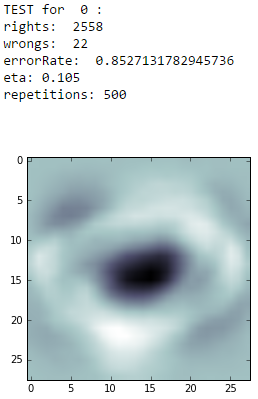
\includegraphics[height=2.6in]{test0}
            \caption*{0 vs all}
		\end{subfigure}%
		~
		\begin{subfigure}[t]{0.32\textwidth}
			\centering
			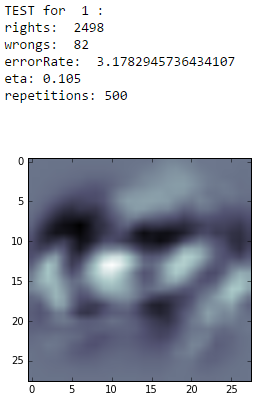
\includegraphics[height=2.6in]{test1}
            \caption*{1 vs all}
		\end{subfigure}
		~
		\begin{subfigure}[t]{0.32\textwidth}
			\centering
			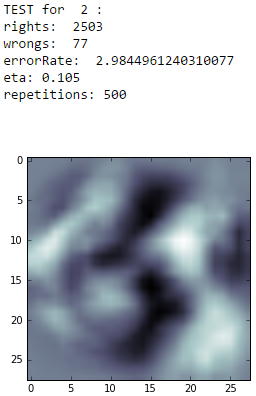
\includegraphics[height=2.6in]{test2}
            \caption*{2 vs all}
		\end{subfigure}
		~
		\begin{subfigure}[t]{0.32\textwidth}
			\centering
			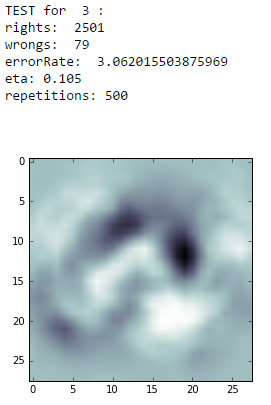
\includegraphics[height=2.6in]{test3}
            \caption*{3 vs all}
		\end{subfigure}%
		~
		\begin{subfigure}[t]{0.32\textwidth}
			\centering
			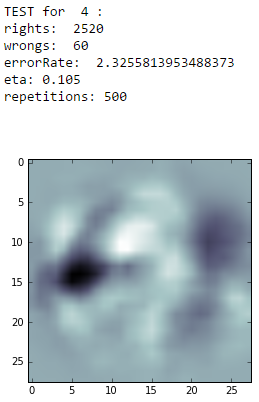
\includegraphics[height=2.6in]{test4}
            \caption*{4 vs all}
		\end{subfigure}
		~
		\begin{subfigure}[t]{0.32\textwidth}
			\centering
			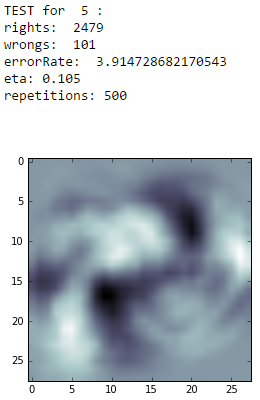
\includegraphics[height=2.6in]{test5}
            \caption*{5 vs all}
		\end{subfigure}
		~
		\begin{subfigure}[t]{0.32\textwidth}
			\centering
			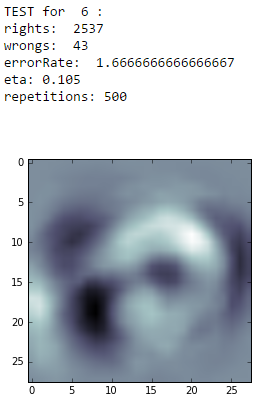
\includegraphics[height=2.6in]{test6}
            \caption*{6 vs all}
		\end{subfigure}%
		~
		\begin{subfigure}[t]{0.32\textwidth}
			\centering
			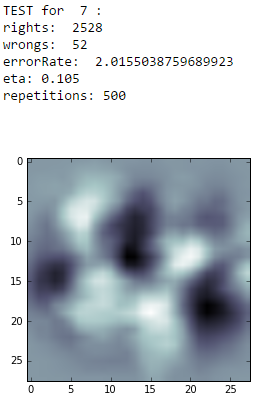
\includegraphics[height=2.6in]{test7}
            \caption*{7 vs all}
		\end{subfigure}
		~
		\begin{subfigure}[t]{0.32\textwidth}
			\centering
			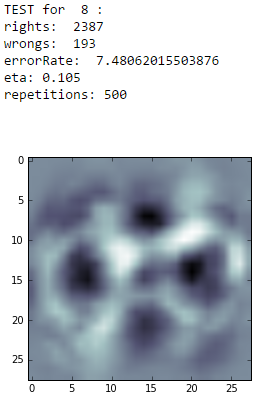
\includegraphics[height=2.6in]{test8}
            \caption*{8 vs all}
		\end{subfigure}
    \end{figure*}
    
    \begin{figure*}
		\begin{subfigure}[t]{0.32\textwidth}
			\centering
			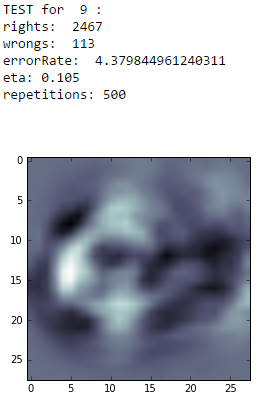
\includegraphics[height=2.6in]{test9}
            \caption*{9 vs all}
		\end{subfigure}%
		~
        \captionsetup{justification=centering}
		\begin{subfigure}[t]{0.5\textwidth}
			\centering
			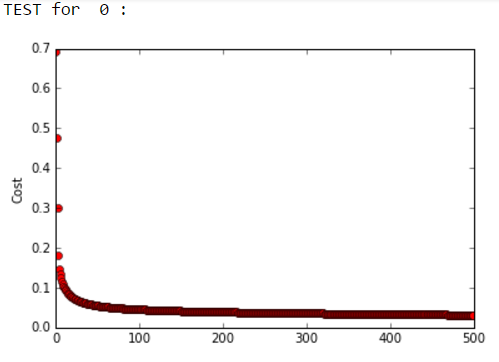
\includegraphics[height=2.6in]{costfun}
            \caption*{Cost function y-axis, steps x-axis. \\
            		  Taken from a 0 vs-all calculation}
		\end{subfigure}
        ~
		\begin{subfigure}[t]{\textwidth}
			\centering
			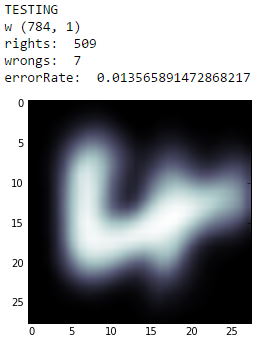
\includegraphics[height=3in]{2vs7}
            \caption*{2 vs 7 with 50.000 runs and a errorRate on 1,35\%}
		\end{subfigure}
	\end{figure*}
    
    \begin{figure*}
   		\begin{subfigure}[t]{\textwidth}
    		\centering
    		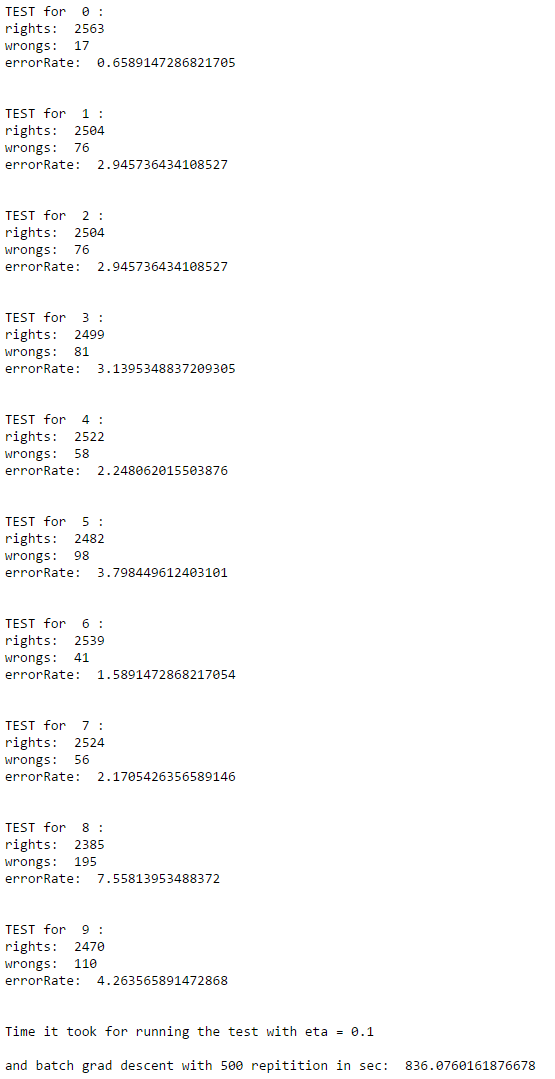
\includegraphics[height=9.5in]{batchrun}
    	\end{subfigure}
    \end{figure*}
    
    \begin{figure*}
    	\begin{subfigure}[t]{\textwidth}
    		\centering
    		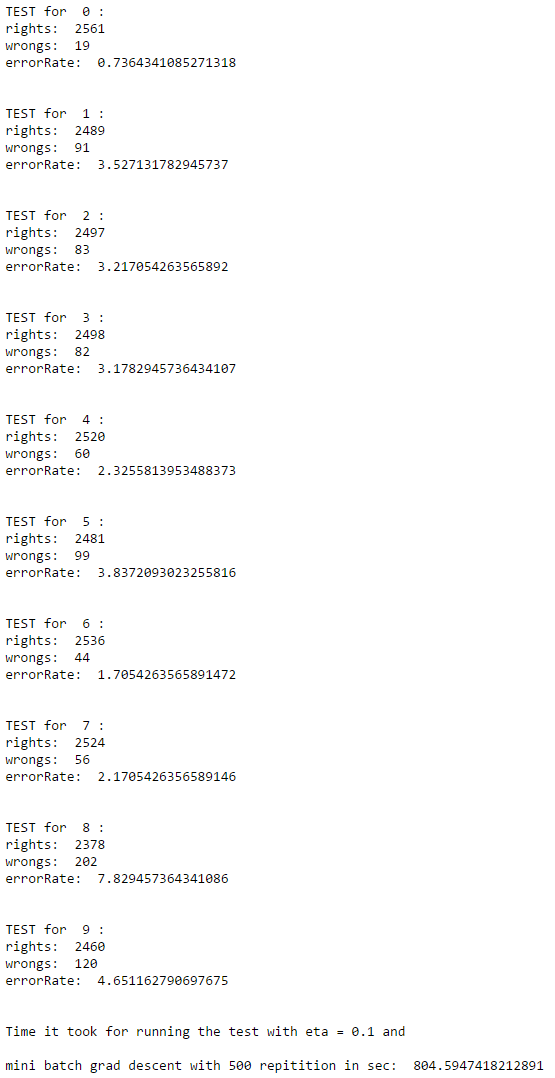
\includegraphics[height=9.5in]{minibatchrun}
    	\end{subfigure}
    \end{figure*}
 
\begin{figure*}
Below there is two pictures of the first 10 numbers that has been misclassified in 4 vs all test. The first is with 10 repetitions and the last is with 1000 repetitions. We can see that in first figure there is a lot of "normal" fours that has been misclassified mainly because of lack of training cycles. This is different from the last figure where it is sixes and sevens that has been seen as fours and then some of the more weird fours that haven't been found. This types of error is because the misclassified numbers are outliers to their own class. They are too different from the average form of the numbers in their class.  \\ \\
    \framebox{
		\begin{subfigure}[t]{\textwidth}
			\centering
            \caption*{10 repetition}
			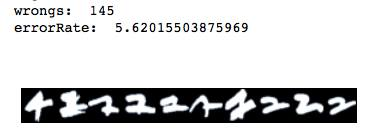
\includegraphics[height=1.9in]{10}
		\end{subfigure}
    } 
    ~
    \newline
	\framebox{
    	\begin{subfigure}[t]{\textwidth}
			\centering
            \caption*{1000 repetition}
			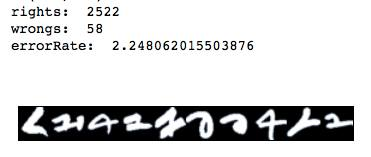
\includegraphics[height=2.4in]{1000}
		\end{subfigure}
    }
\end{figure*}
\newpage
\section{Multinomial/softmax regression}
\subsection{implementation}
In this part of the project we generalize logistic regression to handle 10 classes instead of 2. The implementation is almost the same as before but now the target values is represented by a (n x K) matrix Y which makes the calculations for W, cost and gradient a bit different.

Halfway through this exercise we realized that calculating the cost took way too much time, because we had written it with several for-loops. By using np.sum() it took less time. 
We also realized that because of the size of cost our eta was to small a number. by setting eta to 100, cost got significantly lower in the 50 repetitions we managed to test for.
Due to time constraints, we haven't been able to implement the mini-batch-grad-descent algorithm for the softmax regression, which of cause i unfortunate.

\subsection{performance}
In the cost function plot below we can see that cost converges to a minimum. And in the plot of our W in the softmax run, we can see some nice blurry numbers where the whiteness of a pixel shows the possibility that a number in the given class have been drawn on that pixel. Of course the numbers in this figure are concatenated, such that the square is 0, the next 1, etc. 
\\ \\
Below is the error rate for our best run with softmax, batch-gradient-descent. We see the results are comparable if you would take a mean of the error rates, of the different 1 vs all runs and compare it to the softmax, and this is with one tenth of the iterations as the 1 vs all test, and there we had to run each of them for every number. So we observe that the softmax we about as one vs all, with far fever iteration and much lower running time of 36 sec. Of cause some of this has to come from us learning the library numpy better, and finding 'more clever solutions', but some of also have to come from the much lower iteration number.

\begin{figure*}[!htb]
	\framebox{
    	\begin{subfigure}[t]{\textwidth}
    		\centering
    		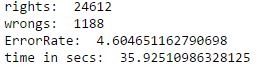
\includegraphics[height=0.5in]{bestsoftmax}
            \caption*{Our best run of softmax}
    	\end{subfigure}
     }
\end{figure*}

	\begin{figure*}[!htb]
    	\begin{subfigure}[t]{\textwidth}
    		\centering
    		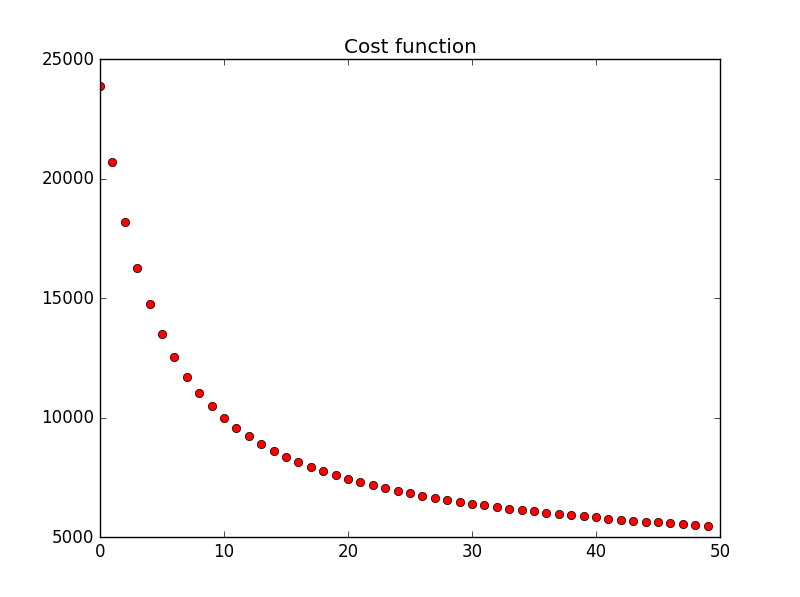
\includegraphics[height=3in]{softcostfun}
            \caption*{Function of cost on each iteration, with eta = 100}
    	\end{subfigure}
        ~
        \newline
        \newline
        \newline
        \begin{subfigure}[t]{\textwidth}
        	\centering
    		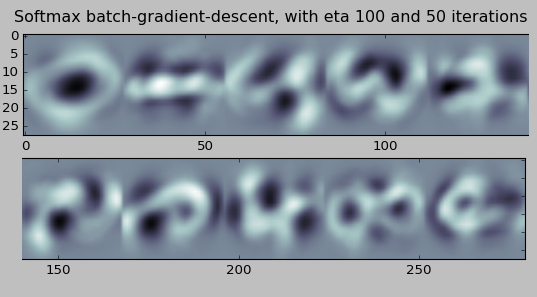
\includegraphics[height=3in]{softmax0-9}
            \caption*{A plot of W}
    	\end{subfigure}
        ~
        \newline
        \newline
        \newline
        \begin{subfigure}[t]{\textwidth}
        	\centering
    		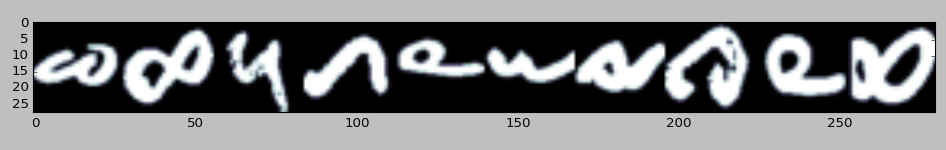
\includegraphics[height=1in]{missclassified}
            \caption*{Miss classified numbers}
    	\end{subfigure}
    \end{figure*}



\end{document}